\documentclass[11pt,a4paper]{article}
\usepackage[utf8]{inputenc}
\usepackage[T1]{fontenc}
\usepackage{graphicx}
\usepackage{booktabs}
\usepackage{hyperref}
\usepackage{amsmath}
\usepackage{siunitx}
\usepackage{geometry}
\usepackage{caption}
\usepackage{subcaption}
\usepackage{float}
\geometry{margin=2.5cm}

\title{CAMPUS 5G Protocol Benchmark --- Follow-up Results\\[0.3em]
\large Adding QUIC Transports and Scaling to 50 Devices}
\author{Samiullah Khairy}
\date{May 29, 2026}

\begin{document}
\maketitle

\section{What this follows up on}

In the previous report (May 26) I benchmarked three protocols --- gRPC, Zenoh, and MQTT over TCP --- across 144 runs and found that MQTT over TCP breaks completely under degraded 5G conditions: median RTT reached 32 seconds at $N=10$ with 1\% packet loss. Zenoh and gRPC both handled it fine, sitting at the 160~ms network floor.

That report ended with two open questions:
\begin{enumerate}
    \item Can swapping TCP for QUIC fix MQTT? QUIC avoids TCP head-of-line blocking, which was identified as the root cause of the queue collapse.
    \item How do the protocols scale beyond $N=10$? The original sweep only went up to 10 devices.
\end{enumerate}

This report answers both. I extended the benchmark to five protocol configurations and scaled up to $N=50$ devices, running a total of 360 experiments.

\section{What changed in the setup}

The containerized testbed, netem impairment profiles, and measurement loop are identical to the previous report. The only additions are two new protocol configurations:

\begin{itemize}
    \item \textbf{Zenoh-over-QUIC} --- the same Zenoh router and client images, reconfigured to use QUIC (UDP) instead of TCP.
    \item \textbf{MQTT-over-QUIC} --- a completely different stack from MQTT over TCP. The broker is NanoMQ (not Mosquitto) with a native QUIC listener. The clients are C binaries compiled against NanoSDK with MsQuic support, running asynchronous callbacks instead of the polling loop the Python \texttt{paho-mqtt} client uses. This eliminates the 45~ms polling floor entirely.
\end{itemize}

I also extended the device count sweep from $N \in \{1, 2, 5, 10\}$ to $N \in \{1, 2, 5, 10, 20, 50\}$, giving the full matrix:

\[
5 \text{ protocols} \times 3 \text{ profiles} \times 6 \text{ device counts} \times 2 \text{ payloads} \times 2 \text{ rates} = \mathbf{360\ runs}
\]

\subsection*{Message volume at scale}

At $N=50$ devices, 10~Hz, 30~s, the edge sends 15,000 commands and receives 15,000 acknowledgements --- 30,000 application-level messages per run. For broker-based protocols (MQTT), each message passes through the broker twice in each direction, giving \textbf{60,000 broker message transitions} per run. This is the load that exposes the architectural limits of each approach.

\section{Results}

\subsection{Baseline: clean network}

\begin{table}[H]
\centering
\caption{Baseline latency on clean network ($N=1$, 100~B, 10~Hz)}
\label{tab:clean}
\begin{tabular}{lrrrr}
\toprule
Protocol & p50 (ms) & p95 (ms) & p99 (ms) & Mean (ms) \\
\midrule
Zenoh-QUIC  & 2.64 & 2.89 & 3.00 & 2.37 \\
Zenoh (TCP) & 2.61 & 2.88 & 2.98 & 2.30 \\
MQTT-QUIC   & 1.95 & 5.36 & 5.65 & 2.68 \\
gRPC        & 3.29 & 3.65 & 4.24 & 2.74 \\
MQTT (TCP)  & 44.02 & 45.97 & 46.19 & 43.90 \\
\bottomrule
\end{tabular}
\end{table}

The first thing that jumps out: MQTT-over-QUIC drops the baseline from \textbf{44~ms to 2~ms}. This confirms that the 45~ms floor I saw in the first report was entirely the \texttt{paho-mqtt} polling delay, not anything intrinsic to the MQTT protocol. The NanoSDK C client with asynchronous callbacks eliminates it completely.

Zenoh and Zenoh-QUIC are essentially identical at baseline --- both sub-3~ms --- which makes sense since on a clean local network QUIC doesn't add anything over TCP.

At $N=50$ on the clean network, Zenoh and Zenoh-QUIC stay below 5~ms (p95). MQTT-QUIC rises to $\sim$20~ms at this scale, which is NanoMQ's per-stream multiplexing showing minor overhead at high concurrency. Interestingly, MQTT TCP's polling floor also disappears at $N=50$ because the broker keeps the client loop continuously busy --- both converge to around 20~ms.

\subsection{Normal 5G conditions}

\begin{table}[H]
\centering
\caption{RTT under normal 5G (2000~B payload, 10~Hz)}
\label{tab:good5g}
\begin{tabular}{lcrrrr}
\toprule
Protocol & $N$ & Loss (\%) & p50 (ms) & p95 (ms) & p99 (ms) \\
\midrule
Zenoh-QUIC  & 10 & 1.1  & 41.69  & 44.22  & 45.66 \\
Zenoh (TCP) & 10 & 1.4  & 42.21  & 44.78  & 46.11 \\
MQTT-QUIC   & 10 & 0.3  & 45.32  & 52.70  & 66.68 \\
gRPC        & 10 & 11.1 & 43.04  & 46.11  & 49.19 \\
MQTT (TCP)  & 10 & 2.7  & 90.48  & 158.10 & 196.04 \\
\midrule
Zenoh-QUIC  & 20 & 1.2  & 41.00  & 43.71  & 45.01 \\
Zenoh (TCP) & 20 & 1.8  & 41.58  & 44.33  & 45.61 \\
MQTT-QUIC   & 20 & 0.3  & 45.39  & 55.68  & 65.16 \\
gRPC        & 20 & 54.9 & 42.67  & 45.84  & 47.78 \\
MQTT (TCP)  & 20 & 1.5  & 460.76 & 792.57 & 933.33 \\
\bottomrule
\end{tabular}
\end{table}

At $N=10$, MQTT-QUIC is now competitive with gRPC and Zenoh --- sitting at 45~ms median, right on the 40~ms network floor. Compare that to MQTT TCP still at 90~ms, carrying the network delay plus the broker overhead.

At $N=20$, two things stand out:

\begin{itemize}
    \item \textbf{gRPC drops 55\% of messages.} The messages that do get through have normal latency ($\sim$43~ms), but more than half never arrive. This is HTTP/2 stream exhaustion under simultaneous fan-out to 20 devices.
    \item \textbf{MQTT TCP is already at 461~ms median} with only 0.1\% packet loss. At 20 devices and 10~Hz, cumulative broker load starts outrunning the drain rate. This will cascade into full collapse under any real packet loss.
\end{itemize}

Zenoh (TCP and QUIC) and MQTT-QUIC scale cleanly to $N=20$ with sub-2\% loss and latency within 5~ms of the network floor.

Figure~\ref{fig:latency_vs_n} shows the p95 latency versus device count. The left panel shows all five protocols so the MQTT TCP divergence is visible in context; the right panel zooms into the four that actually work, where you can see the real differences between them.

\begin{figure}[H]
\centering
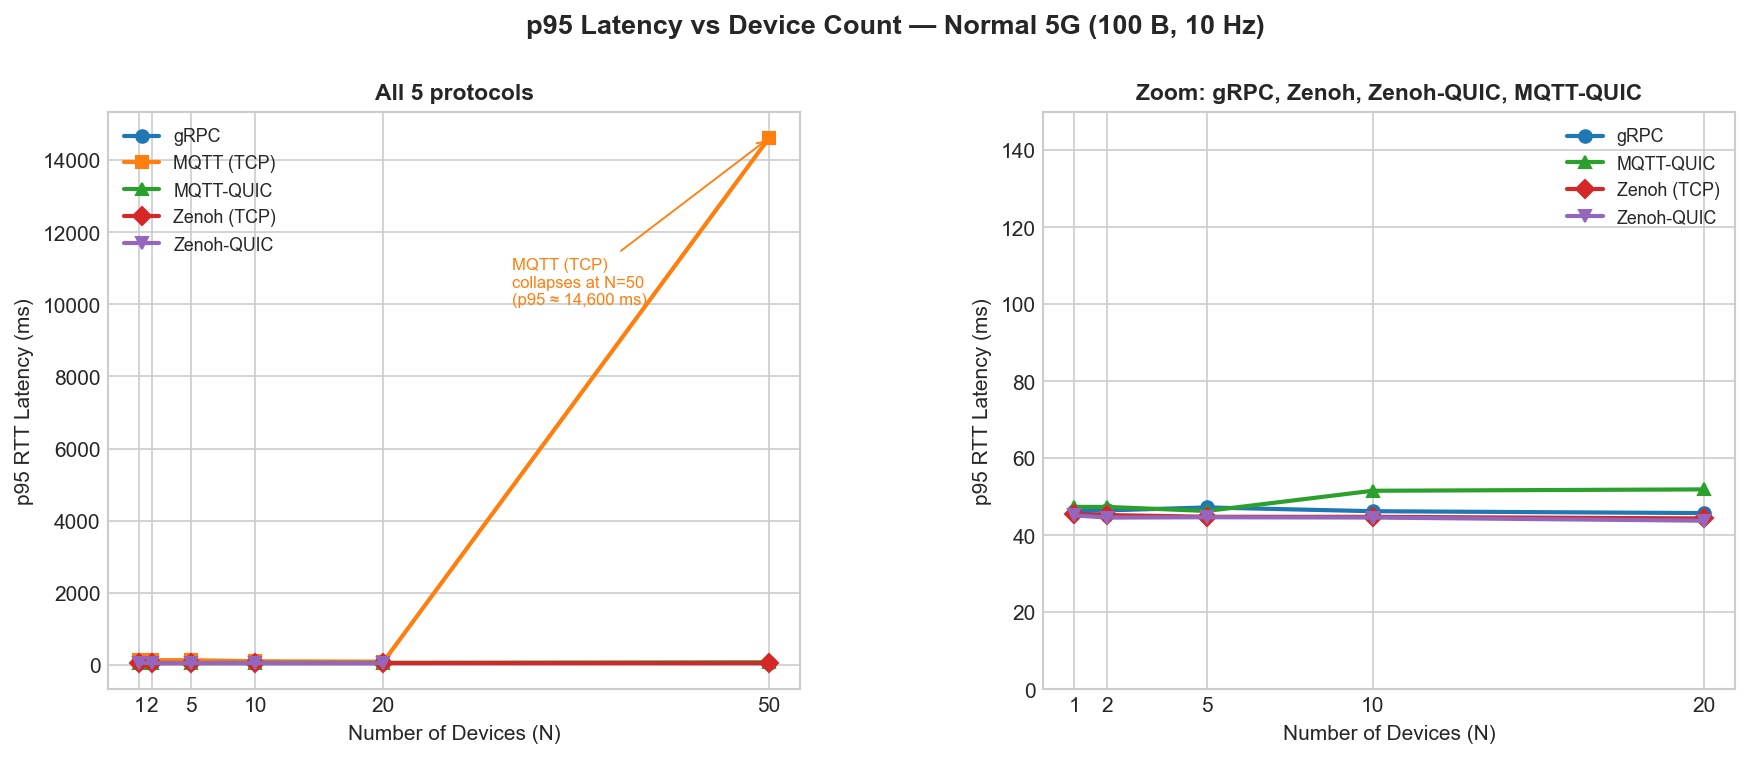
\includegraphics[width=\textwidth]{results/unified/latency_vs_N.png}
\caption{p95 latency vs.\ device count under normal 5G (100~B, 10~Hz). Left: all five protocols --- MQTT TCP diverges at $N=20$ and saturates at $N=50$ (p95 $\approx$ 14,600~ms). Right: zoom on the four viable protocols --- Zenoh, Zenoh-QUIC, and gRPC are flat; MQTT-QUIC rises slightly at higher $N$ but stays well within bounds.}
\label{fig:latency_vs_n}
\end{figure}

\subsection{Degraded 5G --- where the architectures separate}

\begin{table}[H]
\centering
\caption{RTT under degraded 5G (2000~B payload, 10~Hz)}
\label{tab:degraded}
\begin{tabular}{lcrrrr}
\toprule
Protocol & $N$ & Loss (\%) & p50 (ms) & p95 (ms) & p99 (ms) \\
\midrule
Zenoh-QUIC  & 10 & 1.0 & 163.75     & 306.65     & 432.76 \\
Zenoh (TCP) & 10 & 1.4 & 163.22     & 262.93     & 438.20 \\
MQTT-QUIC   & 10 & 0.3 & 210.13     & 371.26     & 486.05 \\
gRPC        & 10 & 8.2 & 164.61     & 229.71     & 433.40 \\
MQTT (TCP)  & 10 & 1.4 & 38{,}759   & 64{,}452   & 67{,}034 \\
\midrule
Zenoh-QUIC  & 20 & 1.0 & 161.50     & 254.37     & 426.78 \\
Zenoh (TCP) & 20 & 1.7 & 161.88     & 255.87     & 425.31 \\
MQTT-QUIC   & 20 & 0.3 & 183.33     & 249.46     & 318.23 \\
gRPC        & 20 & 53.7& 162.13     & 226.50     & 427.80 \\
MQTT (TCP)  & 20 & 2.2 & 86{,}589   & 166{,}654  & 175{,}299 \\
\bottomrule
\end{tabular}
\end{table}

MQTT-QUIC at $N=10$ registers a \textbf{210~ms median} under degraded 5G --- compared to 38,759~ms for MQTT TCP under identical conditions. That is a \textbf{185$\times$ reduction} just from swapping the transport layer.

The root cause is the same one I described in the first report: TCP head-of-line blocking stalls the broker's PUBACK handshake and the queue grows without bound. QUIC eliminates this because each device's stream is independent --- a lost packet on one stream doesn't block any other. The broker queue drains continuously.

At $N=20$, MQTT TCP median reaches \textbf{86.6 seconds} even though only 2.2\% of messages are lost. The queue bloat compounds with device count.

Figure~\ref{fig:degraded_vs_n} shows the median latency scaling under degraded conditions, and Figure~\ref{fig:rescue} isolates the MQTT TCP vs MQTT-QUIC comparison directly.

\begin{figure}[H]
\centering
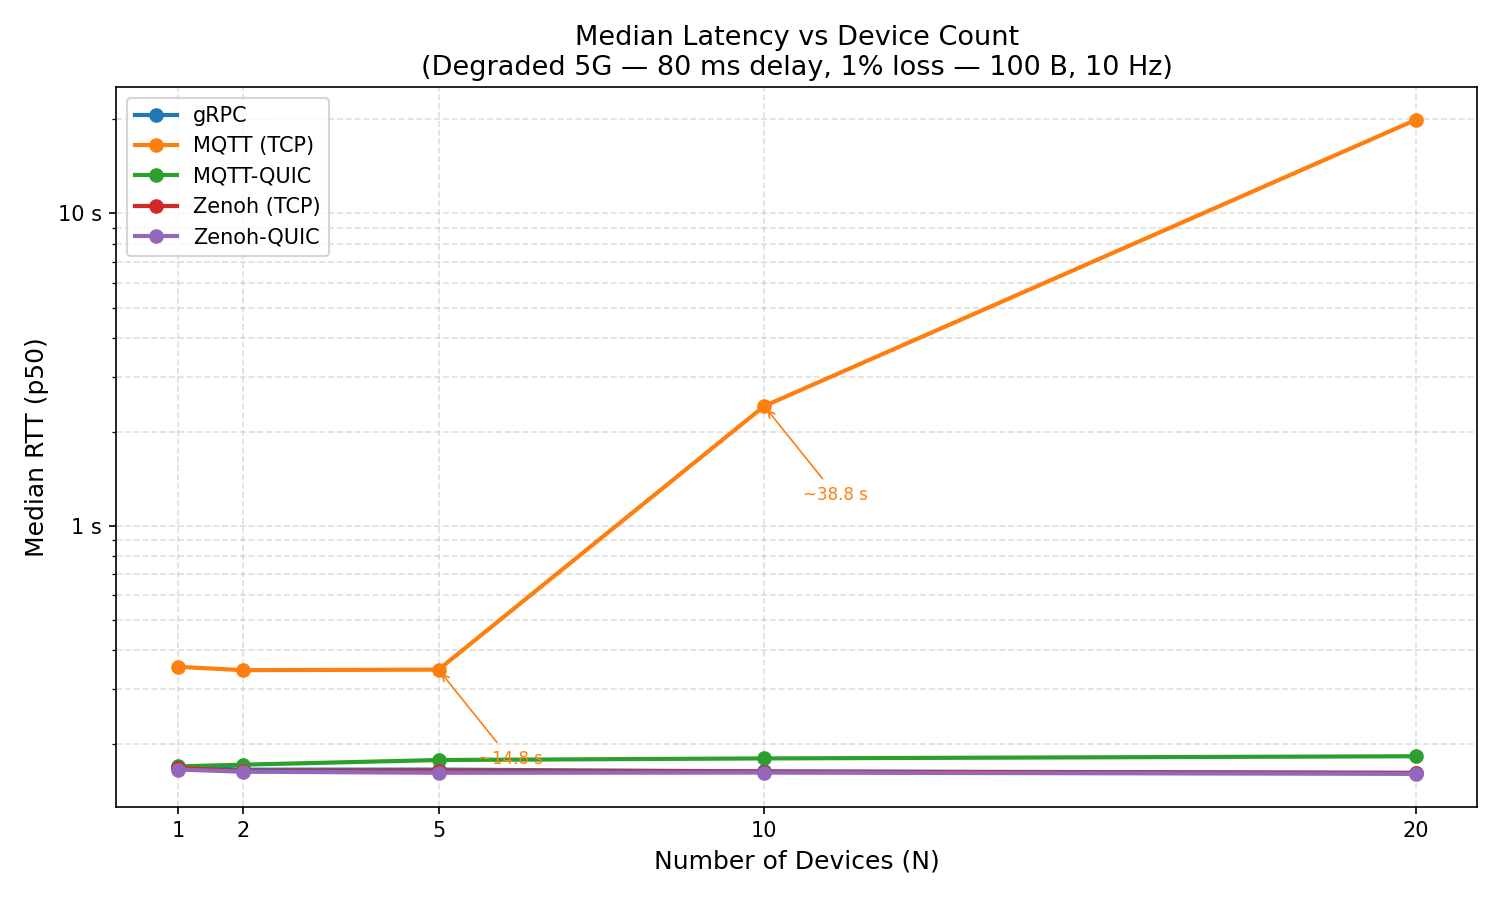
\includegraphics[width=0.82\textwidth]{results/unified/degraded_latency_vs_N.png}
\caption{Median RTT vs device count under degraded 5G (100~B, 10~Hz, log scale). MQTT TCP breaks at $N=5$ (14.8~s) and keeps climbing. All other protocols stay flat between 160~ms and 250~ms across $N=1$ to $N=20$.}
\label{fig:degraded_vs_n}
\end{figure}

\begin{figure}[H]
\centering
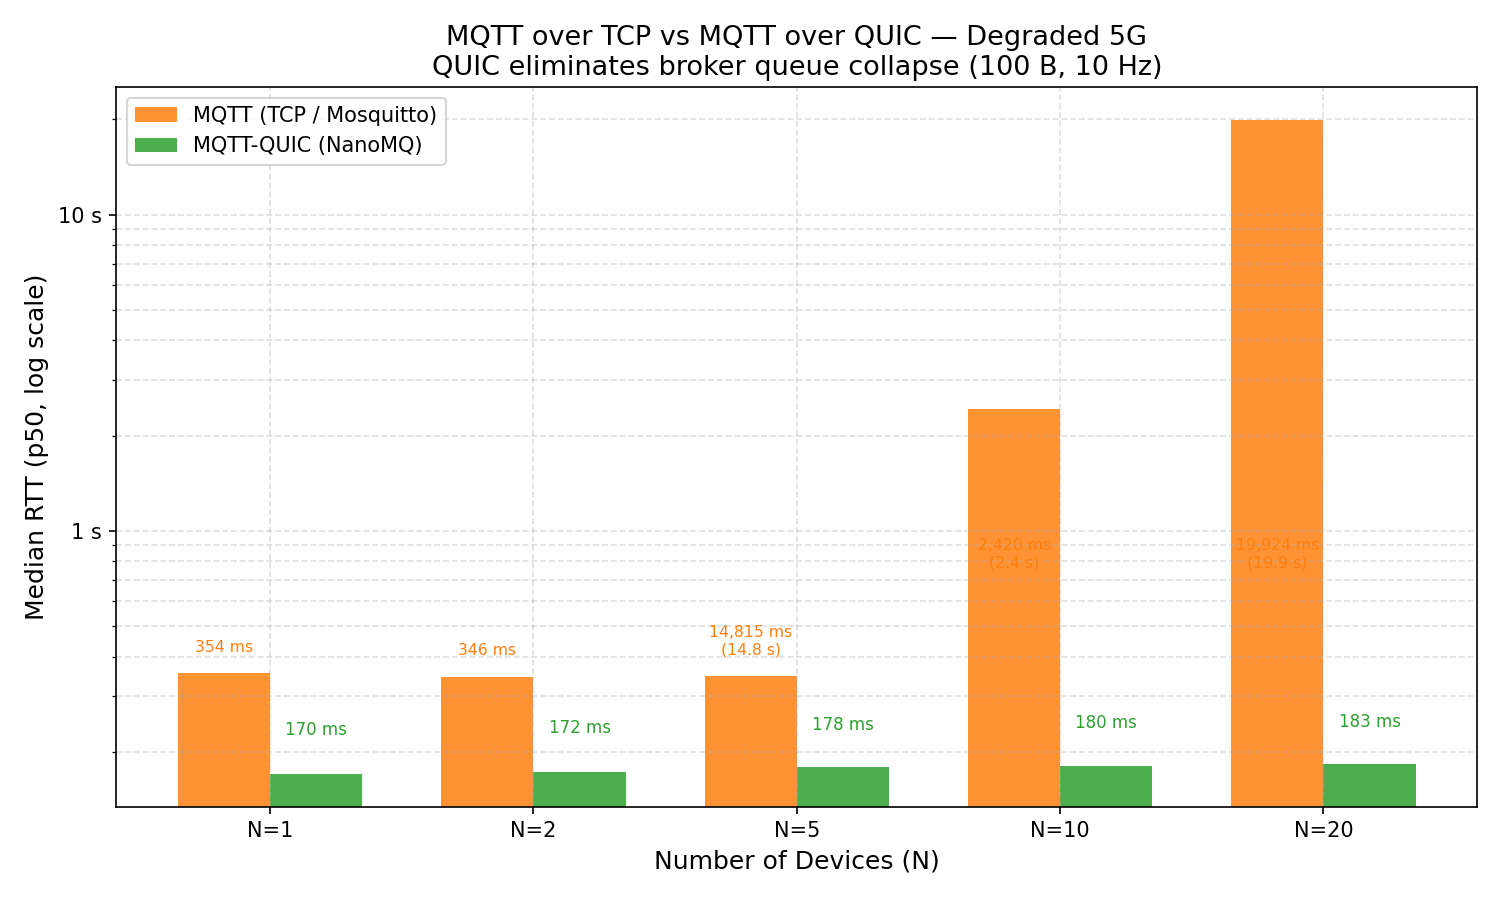
\includegraphics[width=0.82\textwidth]{results/unified/mqtt_quic_rescue.png}
\caption{MQTT TCP vs MQTT-QUIC under degraded 5G (100~B, 10~Hz). Swapping the transport from TCP to QUIC, with no other protocol changes, eliminates the queue collapse entirely.}
\label{fig:rescue}
\end{figure}

\begin{figure}[H]
\centering
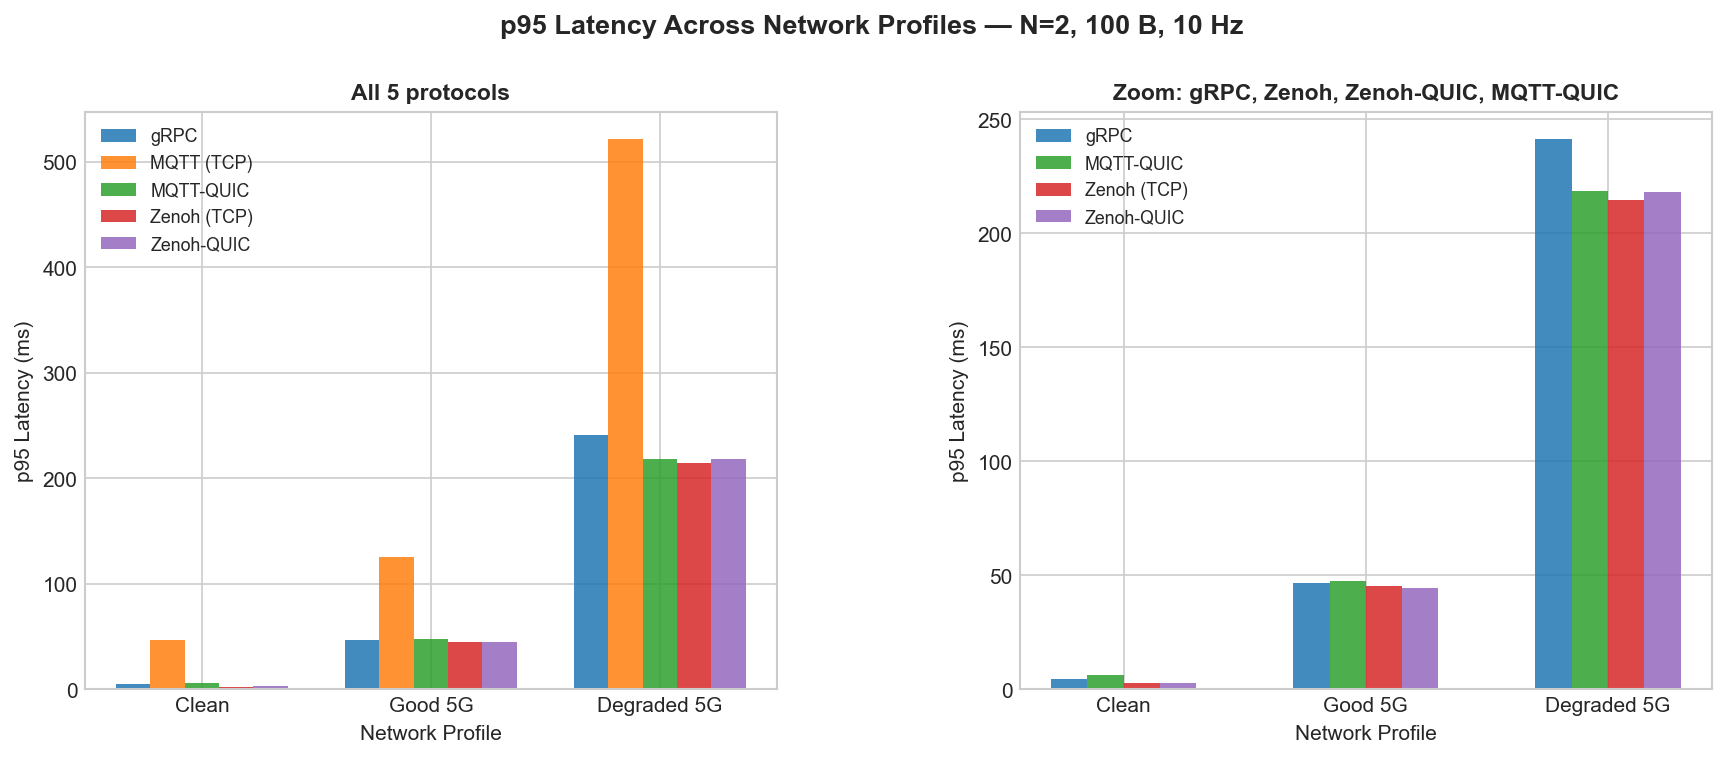
\includegraphics[width=\textwidth]{results/unified/profile_comparison.png}
\caption{p95 latency across all three network profiles ($N=2$, 100~B, 10~Hz). Left: all five protocols. Right: zoom on the four viable ones --- under degraded 5G, Zenoh TCP, Zenoh-QUIC, and MQTT-QUIC cluster tightly at $\sim$215~ms, while gRPC is slightly higher at $\sim$241~ms.}
\label{fig:profile}
\end{figure}

\begin{figure}[H]
\centering
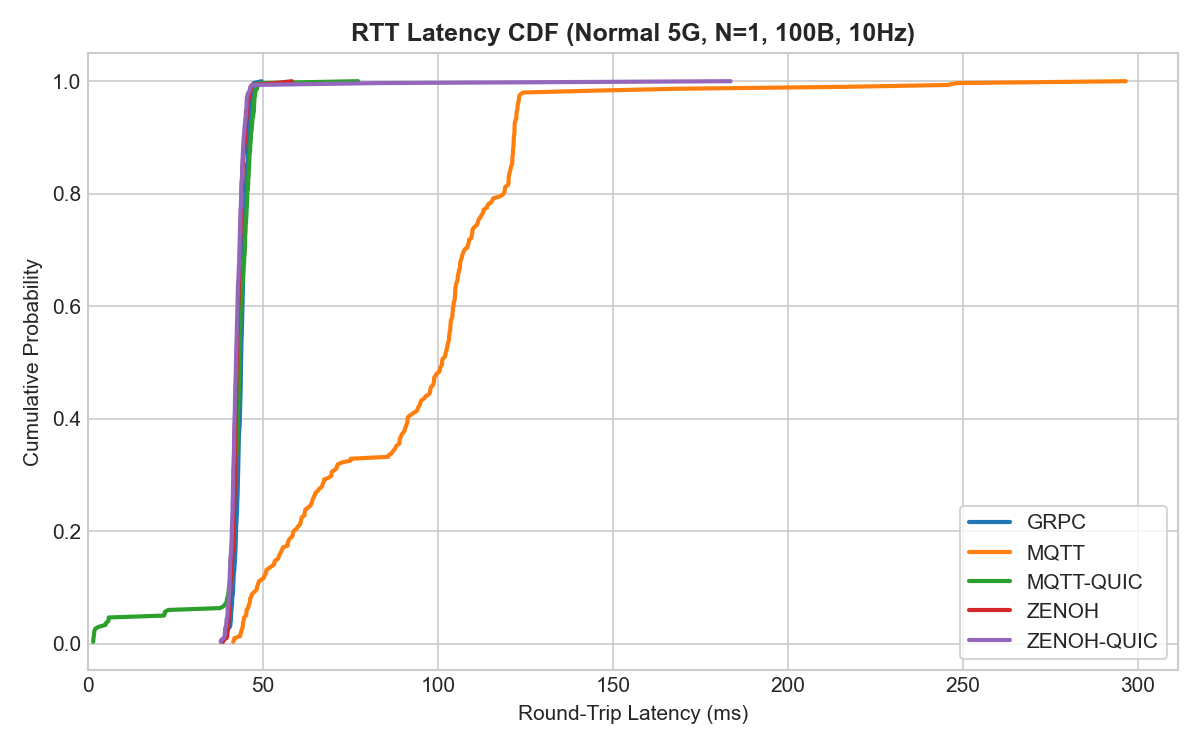
\includegraphics[width=0.75\textwidth]{results/unified/latency_cdf.png}
\caption{RTT latency CDF under normal 5G ($N=1$, 100~B, 10~Hz). MQTT TCP is shifted right by $\sim$45~ms. Zenoh, Zenoh-QUIC, and MQTT-QUIC all cluster at the 43~ms network floor.}
\label{fig:cdf}
\end{figure}

\section{What this means for CAMPUS}

Table~\ref{tab:summary} summarises the five protocols at $N=10$, which is the most representative scale for the current lab setup.

\begin{table}[H]
\centering
\caption{Protocol comparison at $N=10$, 2000~B payload, 10~Hz}
\label{tab:summary}
\begin{tabular}{lrrrrl}
\toprule
Protocol & Clean p50 & Normal 5G p50 & Degraded p50 & Msg loss & Scales to $N=20$? \\
\midrule
Zenoh-QUIC  & 2.7~ms & 42~ms & 164~ms       & $<$2\%   & Yes \\
Zenoh (TCP) & 2.6~ms & 42~ms & 163~ms       & $<$2\%   & Yes \\
MQTT-QUIC   & 4.9~ms & 45~ms & 210~ms       & $<$1\%   & Yes \\
gRPC        & 3.3~ms & 43~ms & 165~ms       & 8--11\%  & No (55\% loss at $N=20$) \\
MQTT (TCP)  & 44~ms  & 90~ms & 38{,}759~ms  & 1--3\%   & No (queue collapse) \\
\bottomrule
\end{tabular}
\end{table}

Based on these results, my recommendations are:

\begin{enumerate}
    \item \textbf{Don't use MQTT over TCP for any real-time loop.} It was already disqualified in the first report and the scaling results confirm it. At $N=20$ under degraded conditions, the median latency is 86 seconds.

    \item \textbf{Zenoh-over-QUIC is the primary recommendation for the pub/sub layer.} Lowest baseline overhead, flat latency to $N=20$, best performance under both normal and degraded conditions, and the topic-based filtering maps directly to the ROI-based selective downlink we need for CAMPUS.

    \item \textbf{MQTT-over-QUIC is the right choice if a central broker is needed.} For example, if the Torino integration requires EMQX or a standard broker for CAMARA API compatibility. QUIC keeps it viable: 210~ms median at $N=10$ under degraded 5G, clean scaling to $N=20$.

    \item \textbf{gRPC for point-to-point transfers only.} HD map streaming, bulk uploads from UE to edge --- anything where a direct connection with flow control makes sense. Not suitable as a broadcast protocol.
\end{enumerate}

\section{Limitations and next steps}

\begin{itemize}
    \item The network impairment is still synthetic (\texttt{tc netem} on a Docker bridge). The next step is to run this on the lab's physical 5G testbed to validate the protocol rankings hold with real radio. I'm planning to start with Open5GS + UERANSIM to get familiar with the 5G deployment workflow before moving to the physical setup.

    \item Each configuration was run once for 30 seconds. For a publication-quality result, I'd run each 3--5 times and report median with confidence intervals.

    \item I didn't profile CPU or memory consumption of the containers. QUIC processing happens in user space and may carry higher CPU overhead than kernel-space TCP at production scale --- this is unmeasured.

    \item At $N=50$, several Zenoh and Zenoh-QUIC runs returned no data (header-only CSV files), indicating the router container hit a resource limit in the Docker environment. The $N \leq 20$ data is clean and sufficient for the architecture decision; $N=50$ should be revisited on the physical testbed.
\end{itemize}

\end{document}
